\chapter{铁碳合金的显微组织观察及性能分析}
\section{实验目的}
    \begin{enumerate}
        \item 了解金相分析基本概念。
        \item 掌握碳钢金相试样的制备方法及显微组织的显示方法。
        \item 按金相试样流程制备1个碳钢金相试样,并观察和分析其显微组织。
    \end{enumerate}
\section{实验原理}%简单描述,含必要的公式和附图;
    \subsection{金相试样的磨光}
    磨光是制备金相试样的关键性工序。磨光分为粗摩和细摩。粗摩的目的是平整试样表面,同时去除掉截取试样所产生的应力变形层,为细磨做准备。\textbf{磨光的第一个步骤应对试样磨面的边缘进行倒角},以防后道工序中,尖角、棱角划破砂纸及抛光布,甚至划伤手指。经粗磨后的试样表面虽较平整,但仍存在有较深的磨痕。细磨的目的就是为了消除这些磨痕,得到平整而光滑的磨面,并为进一步的抛光做好准备。
        \subsubsection{手工磨光}
        手工磨光是在由粗到细的各号金相砂纸上进行。砂纸上的磨料一般是碳化硅或氧化铝微粉。砂纸平铺在玻璃、金属、塑料或木板等光滑平板上,磨制过程中操作人员需一手紧压砂纸,另一手平稳地拿住试样,将磨面轻压砂纸,向前平推,然后提起、拉回,拉回时试样勿与砂纸接触,不可来回磨削,否则磨面易成弧形,不易得到平整的磨面。
        \subsubsection{金相试样的抛光}
        抛光的目的是为了清除最细一号砂纸磨光后试详表面所留下的细微磨痕,使试样的磨面成为光滑无痕的镜面。\par
        常用的抛光方法有机械抛光、电解抛光与化学抛光三类。本实验只介绍机械抛光法。机械抛光是在抛光机的转盘上进行的,转盘上盖有抛光织物。整个过程中还需抛光磨料配合进行抛光。
        \subsubsection{金相显微组织的显示}
        显示金相组织的方法很多,最常用的是化学浸蚀法和电解浸蚀法,还有一些特殊显示方法(如热染、热蚀、阴极真空显示磁性显示等),本实验只介绍化学浸蚀法。化学浸蚀法是用化学试剂溶解试样的化学作用来显示其金相显微组织的。对于纯金属及单相合金,化学试剂溶液的浸蚀作用是一种纯粹的化学溶解过程,磨面表层的原子被溶入浸蚀剂中。在溶解过程中,由于晶粒与晶粒之间,晶粒与晶界之间溶解速度的不同,组织就被显示出来,漫蚀剂首先把磨面表层的变形层(非晶形层)溶去,接着就对晶界起化学溶解作用。因为在晶界上原子排列的规律性较差,这部分原子具有较高的自由能,最易被浸蚀溶解,因此在化学浸蚀时,晶界首先被显示出来(如\fgref{fig:jingjie}),若浸蚀继续进行,则浸蚀剂将对晶粒本身起溶解作用,由于磨面上每个晶粒原子排列的位向不同,不同的晶面溶解速率不同,浸蚀以后的显微平面与原磨面的角度不同,也就是说每个晶粒被浸蚀后的平面与原来的磨面倾斜了一定的角度。于是,在垂直光线照射下,反射进入物镜的光线不同,就可以看到明暗不同的晶粒。
        \begin{figure}[!ht]
            \caption{晶界的显示\label{fig:jingjie}}
            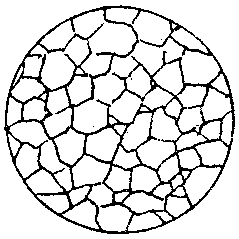
\includegraphics[width=0.28\textwidth]{img/A2/jingjie.png}
        \end{figure}
        \subsubsection{化学浸蚀操作}
        化学浸蚀是否成功取决于作用的浸蚀剂、浸蚀方法和浸蚀时间等因素是否恰当。磨面在浸蚀前必须冲洗清洁,用酒精去除油污,以免阻碍浸蚀。浸蚀操作有两种方法:浸入法及擦拭法。我们采用擦拭法,即用蘸有浸蚀剂的棉花在磨面上轻轻擦拭,因为一般浸蚀的时间都很短,用这种方法比较容易控制,擦拭动作要迅速,并注意观察磨面上光泽的变化,浸蚀时间的长短随浸蚀剂及试样而不同,要视具体情况而定,浸蚀好后,要立即用洒精擦拭并吹干,然后进行显微观察。若显微组织没有完全显示出来,必然是浸蚀过浅,可再继续浸蚀;如果组织色调过于灰黑,失去应用的衬度,则为浸蚀过度,纠正的方法是重新抛光,甚至再用细号砂纸重磨;如果浸蚀后组织模糊不清,不能代表合金的正常组织,这说明磨面表层的非晶形层仍然存在,需经多次洗涤抛光浸蚀,交替操作以除去之。\par
        试样制备完毕后,要注意保护磨面,切忌与其他物件碰擦。在不观察时,一般将制备好的试样放在干燥器内保存,以防止氧化生锈。
\section{实验仪器}%规格及参数
    MDS400 金相显微镜、金相预磨机、金相抛光机、金相砂纸、玻璃板、抛光膏、4\% 硝酸酒精、75\% 酒精、吹风筒、脱指棉球、竹镊子等。
\section{实验过程}%简述主要过程和实验内容
    \subsection{实验内容}
        \begin{enumerate}
            \item 领取试样、并选择不同型号砂纸共 6 张;
            \item 按要求进行磨光、抛光和浸蚀;
            \item 在金相显微镜下检查所制备的金相试样的质量。
        \end{enumerate}
    \subsection{实验内容}
        \begin{enumerate}
            \item 写出金相样品的制备步骤;
            \item 分析制样中出现的问题,并提出改进措施;
            \item 掌握金相样品制备的基本技能,能够制备出基本符合要求的金相样品。
        \end{enumerate}
\section{实验结果}
    \subsection{金相样品的制备步骤}
        制备要经历如下几个步骤:
        \begin{enumerate}
            \item 使用 320 目的砂纸倒角和粗磨。
            \item 使用 400、600、800、1000、1200、1500 目的砂纸磨光,确保每一步的划痕方向一致,并且将上一步的划痕全部磨去。
            \item 使用抛光膏将样品表面抛光成镜面并将划痕全部除去。
            \item 使用4\% 硝酸酒精腐蚀样品表面。
        \end{enumerate}
    \subsection{存在的问题}
    \begin{enumerate}
        \item 力度控制不好,容易将样品磨出多面。解决方法:制样时更加细心。
        \item 抛光时无法将划痕完全除去。解决方法:使用砂纸磨光时注意将上步划痕除去。
    \end{enumerate}
\section{思考题}
\begin{enumerate}
    \item \thinking{分析你所制备的金相试样的质量,总结制样过程中的经验教训。}{大体上符合要求,有少量细划痕,晶界清晰,没有过腐蚀。经验:磨光时可以更加小心,避免不可通过抛光除去的划痕。}
\end{enumerate}